\documentclass[preprint, 3p,
authoryear]{elsarticle} %review=doublespace preprint=single 5p=2 column
%%% Begin My package additions %%%%%%%%%%%%%%%%%%%

\usepackage[hyphens]{url}

  \journal{Transport Geography?} % Sets Journal name

\usepackage{graphicx}
%%%%%%%%%%%%%%%% end my additions to header

\usepackage[T1]{fontenc}
\usepackage{lmodern}
\usepackage{amssymb,amsmath}
% TODO: Currently lineno needs to be loaded after amsmath because of conflict
% https://github.com/latex-lineno/lineno/issues/5
\usepackage{lineno} % add
\usepackage{ifxetex,ifluatex}
\usepackage{fixltx2e} % provides \textsubscript
% use upquote if available, for straight quotes in verbatim environments
\IfFileExists{upquote.sty}{\usepackage{upquote}}{}
\ifnum 0\ifxetex 1\fi\ifluatex 1\fi=0 % if pdftex
  \usepackage[utf8]{inputenc}
\else % if luatex or xelatex
  \usepackage{fontspec}
  \ifxetex
    \usepackage{xltxtra,xunicode}
  \fi
  \defaultfontfeatures{Mapping=tex-text,Scale=MatchLowercase}
  \newcommand{\euro}{€}
\fi
% use microtype if available
\IfFileExists{microtype.sty}{\usepackage{microtype}}{}
\usepackage[]{natbib}
\bibliographystyle{plainnat}

\usepackage{graphicx}
\ifxetex
  \usepackage[setpagesize=false, % page size defined by xetex
              unicode=false, % unicode breaks when used with xetex
              xetex]{hyperref}
\else
  \usepackage[unicode=true]{hyperref}
\fi
\hypersetup{breaklinks=true,
            bookmarks=true,
            pdfauthor={},
            pdftitle={Leveraging GTFS data to assess transit supply},
            colorlinks=false,
            urlcolor=blue,
            linkcolor=magenta,
            pdfborder={0 0 0}}

\setcounter{secnumdepth}{5}
% Pandoc toggle for numbering sections (defaults to be off)

% Pandoc syntax highlighting
\usepackage{color}
\usepackage{fancyvrb}
\newcommand{\VerbBar}{|}
\newcommand{\VERB}{\Verb[commandchars=\\\{\}]}
\DefineVerbatimEnvironment{Highlighting}{Verbatim}{commandchars=\\\{\}}
% Add ',fontsize=\small' for more characters per line
\usepackage{framed}
\definecolor{shadecolor}{RGB}{248,248,248}
\newenvironment{Shaded}{\begin{snugshade}}{\end{snugshade}}
\newcommand{\AlertTok}[1]{\textcolor[rgb]{0.94,0.16,0.16}{#1}}
\newcommand{\AnnotationTok}[1]{\textcolor[rgb]{0.56,0.35,0.01}{\textbf{\textit{#1}}}}
\newcommand{\AttributeTok}[1]{\textcolor[rgb]{0.13,0.29,0.53}{#1}}
\newcommand{\BaseNTok}[1]{\textcolor[rgb]{0.00,0.00,0.81}{#1}}
\newcommand{\BuiltInTok}[1]{#1}
\newcommand{\CharTok}[1]{\textcolor[rgb]{0.31,0.60,0.02}{#1}}
\newcommand{\CommentTok}[1]{\textcolor[rgb]{0.56,0.35,0.01}{\textit{#1}}}
\newcommand{\CommentVarTok}[1]{\textcolor[rgb]{0.56,0.35,0.01}{\textbf{\textit{#1}}}}
\newcommand{\ConstantTok}[1]{\textcolor[rgb]{0.56,0.35,0.01}{#1}}
\newcommand{\ControlFlowTok}[1]{\textcolor[rgb]{0.13,0.29,0.53}{\textbf{#1}}}
\newcommand{\DataTypeTok}[1]{\textcolor[rgb]{0.13,0.29,0.53}{#1}}
\newcommand{\DecValTok}[1]{\textcolor[rgb]{0.00,0.00,0.81}{#1}}
\newcommand{\DocumentationTok}[1]{\textcolor[rgb]{0.56,0.35,0.01}{\textbf{\textit{#1}}}}
\newcommand{\ErrorTok}[1]{\textcolor[rgb]{0.64,0.00,0.00}{\textbf{#1}}}
\newcommand{\ExtensionTok}[1]{#1}
\newcommand{\FloatTok}[1]{\textcolor[rgb]{0.00,0.00,0.81}{#1}}
\newcommand{\FunctionTok}[1]{\textcolor[rgb]{0.13,0.29,0.53}{\textbf{#1}}}
\newcommand{\ImportTok}[1]{#1}
\newcommand{\InformationTok}[1]{\textcolor[rgb]{0.56,0.35,0.01}{\textbf{\textit{#1}}}}
\newcommand{\KeywordTok}[1]{\textcolor[rgb]{0.13,0.29,0.53}{\textbf{#1}}}
\newcommand{\NormalTok}[1]{#1}
\newcommand{\OperatorTok}[1]{\textcolor[rgb]{0.81,0.36,0.00}{\textbf{#1}}}
\newcommand{\OtherTok}[1]{\textcolor[rgb]{0.56,0.35,0.01}{#1}}
\newcommand{\PreprocessorTok}[1]{\textcolor[rgb]{0.56,0.35,0.01}{\textit{#1}}}
\newcommand{\RegionMarkerTok}[1]{#1}
\newcommand{\SpecialCharTok}[1]{\textcolor[rgb]{0.81,0.36,0.00}{\textbf{#1}}}
\newcommand{\SpecialStringTok}[1]{\textcolor[rgb]{0.31,0.60,0.02}{#1}}
\newcommand{\StringTok}[1]{\textcolor[rgb]{0.31,0.60,0.02}{#1}}
\newcommand{\VariableTok}[1]{\textcolor[rgb]{0.00,0.00,0.00}{#1}}
\newcommand{\VerbatimStringTok}[1]{\textcolor[rgb]{0.31,0.60,0.02}{#1}}
\newcommand{\WarningTok}[1]{\textcolor[rgb]{0.56,0.35,0.01}{\textbf{\textit{#1}}}}

% tightlist command for lists without linebreak
\providecommand{\tightlist}{%
  \setlength{\itemsep}{0pt}\setlength{\parskip}{0pt}}




\usepackage{booktabs}
\usepackage{longtable}
\usepackage{array}
\usepackage{multirow}
\usepackage{wrapfig}
\usepackage{float}
\usepackage{colortbl}
\usepackage{pdflscape}
\usepackage{tabu}
\usepackage{threeparttable}
\usepackage{threeparttablex}
\usepackage[normalem]{ulem}
\usepackage{makecell}
\usepackage{xcolor}



\begin{document}


\begin{frontmatter}

  \title{Leveraging GTFS data to assess transit supply}
    \author[Public Transport Research Group (PTRG)]{James Reynolds%
  \corref{cor1}%
  \fnref{1}}
   \ead{james.reynolds@monash.edu} 
    \author[Public Transport Research Group (PTRG)]{Yanda Qu%
  %
  \fnref{2}}
   \ead{yanda.qu@monash.edu} 
    \author[Public Transport Research Group (PTRG)]{Graham Currie%
  %
  \fnref{3}}
   \ead{graham.currie@monash.edu} 
      \affiliation[Public Transport Research Group (PTRG)]{
    organization={Public Transport Research Group (PTRG), Institute of
Transport Studies, Department of Civil Engineering Engineering, Monash
University},addressline={Clayton
Campus},city={Melbourne},postcode={3800},state={Victoria},country={Australia},}
    \cortext[cor1]{Corresponding author}
    \fntext[1]{Research Fellow}
    \fntext[2]{PhD Strudent}
    \fntext[2]{Professor}
  
  \begin{abstract}
  This is the abstract.

  It consists of two paragraphs.
  \end{abstract}
    \begin{keyword}
    keyword1 \sep 
    keyword2
  \end{keyword}
  
 \end{frontmatter}

\hypertarget{introduction}{%
\section{Introduction}\label{introduction}}

``If you can't measure it, you can't manage it'' is often
miss-attributed to \citet{Deming1993new}, who was trying to make the
opposite point \citep{Berenson2016in}. Regardless, service level
indicators are important in researching, managing and seeking to improve
transit operations \citep{FieldingGordonJ1987Mpts, Ryus:2003aa}. Many
indicators already exist including, for example: those in the Transit
Capacity and Quality of Service Manual (TCQSM)\citep{TCQSM:2013} and the
Transit Score metric \citep{WalkScore:2023tg}.

However, practitioners, researchers and advocates using such metrics may
face two inter-related challenges: (1) calculating the metrics
themselves for a specific location and service pattern; and (2)
explaining the metrics, their meaning and importance to those who are
not specialists in transit For example: the TCQSM metrics might be
difficult to calculate without specialist software and data, but, they
use an A to F scoring system and there is an entire guidebook explaining
each;\\
in contrast, entering an address into the Transit Score website will
return a score out of 100 reflecting the quantity of transit available,
but the methodolgy and algorithm is not publicly available, so these
cannot be calculated independently.

Previous research by \citet{currie2007identifying} developed a transit
Supply Index (SI) that appears to be both relatively easy to calculate
and explain to non-transport professionals. It is obtained by
calculating the number of transit arrivals at each stop within an area
of interest, with an adjustment made to account for the typical walking
distance catchment of transit stops and stations. Higher SI scores
indicate areas with higher frequency services and/or better coverage.

Unfortunately, the SI does not appear to have been widely used, perhaps
in part because at the time it was first published timetable data was
not publicly available in a standardized and machine-readable format.
The scores reported in Currie and Senbergs (2007) were calculated
directly from a database of services provided by the transit authority
in Melbourne, Australia. Since then, however, the General Transit Feed
Specification (GTFS) has developed as a way to publish timetable data in
a standardized format.\\
More than 10,000 agencies are now providing GTFS feeds\footnote{There
  are two forms: GTFS-static consisting of the timetable data (the
  scheduled services); and GTFS-realtime, which includes vehicle
  arrivals and departure times based on real-world position data. This
  paper and project uses only the GTFS-static (timetable) format.}
\citep{GTFS}, and many visualization, processing and analysis tools are
now available.

A gap, however, is that there is not yet a tool to calculate SI scores
directly from GTFS datasets. This provides the motivation for the
research reported in this paper, in which a new R package
(gtfssupplyindex) specifically developed to calculate SI scores is
presented. The remainder of this paper is structured as follows: the
next seciton outlines the background to this research, including the
original formulation of the Transit Supply Index, and an explanation of
the GTFS. Section 3 then describes the study methodology, followed by a
brief presentation of results in Section 4. Section 5 discusses the
results, outlines directions for future research and provides a
conclusion.

\hypertarget{background}{%
\section{Background}\label{background}}

\hypertarget{transit-metrics}{%
\subsection{Transit metrics}\label{transit-metrics}}

Even a brief search reveals many metrics available for benchmarking
transit services. Examples include: (1) those in the Transit Cooperative
Research Program (TCRP) Report 88, which is an extensive guidebook on
developing a performance-measurement system \citep{Ryus:2003aa}; (2)
online databases provided by the Florida Transit Information System
(FTIS) \citep{Florida-Transit-Information-System:2018aa} and
\citet{UITP:2015aa}; (3) those used in the extensive annual benchmarking
program undertaken yearly by the Transport Strategy Centre, which
includes over 100 transit providers around the world
\citep{Imperial-College-London:2023aa}; and (4) a recently developed
methodology to calculate `blank spots' within an area, being those
places beyond 400/800 metre walking distances to/from bus and tram
stops/train stations \citep{AlamriSultan2023GAoA}.

The Fielding Triangle \citep{FieldingGordonJ1987Mpts} provides a
framework for understanding how such metrics combine service inputs,
outputs and consumption.\\
to describe cost efficiency and effectiveness; and service
effectiveness. At a larger scale, \citet{Litman:2003ab} and
\citet{Litman:2016aa} discuss some of the traffic, mobility,
accessibility, social equity, strategic planning and other rational
decision-making-based perspectives underling such transit metrics, while
\citet{Reynolds:2017ah} extends these into models of how
institutionalism, incrementalism and other public policy analysis
concepts might apply to decision-making processes. Further examples
include: (1) \citet{GuzmanLuisA.2017Aeit}, who develop a measure of
accessibility in the context of policy development and social equity for
Latin American Bus Rapid Transit (BRT) networks; and (2) the street
space allocation metrics based around 10 ethical principles introduced
by \citet{Creutzig2020streetspaceallocation}.

However, many of these metrics appear difficult to calculate, complex to
explain or understand, and likely not well suited to communication with
those who are not transit planners or engineers, or other technical
specialists. Where pre-calculated metrics are immediately available it
may not be possible for practitioners, researchers or advocates to
independently generate metrics for proposed system changes. Sometimes it
is not even possible to know precisely how scores for the existing
services levels are calculated.

For example, Transit Scores for locations with a published GTFS feed are
readily available on the \citet{WalkScore:2023tg} website, eliminating
the need for any calculations. The meaning of these Transit Scores
appears easy to explain, as the highest possible score of 100 represents
what might be experienced in the centre of New York. However, the
Transit Score algorithm is patented and effectively a black box. It is
not possible to calculate Transit Scores scores independently. Nor can
Transit Scores to be generated for proposed changes to networks. The
Transit Score metric, therefore, fails the first of the aforementioned
challenges, as practitioners, researchers and advocates can only use
those scores provided online. The metric is simple to explain: the
closer to 100, the better; but, because it is based on a patented
algorithm it may not be easy to understand or explain the connection
between real-world conditions and the Transit Score, or what might need
to be done to improve the score (and service levels). As such, it might
partially pass the second of the aforementioned challenges, as it is
simple to understand, yet may not withstand scrutiny.

In contrast, the TCQSM, specifies Levels of Service (LOS) between A and
F across a range of factors\footnote{ Including service span, frequency,
  speed, the proportion of the population serviced, competitiveness of
  travel times to car-based travel, and many more.}. This scoring scheme
appears relatively simple to explain\footnote{ A is good and F is bad.}
and matches that often used in traffic capacity analysis. Detail within
\citet{TCQSM:2013} provides a resource for anyone wanting to better
understand what the scores mean. However, calculation of many of TCQSM
metrics may need specialised software and datasets\footnote{ For
  example, the Service Coverage Area metric in the TCQSM (pp.~5-8 to
  5-21) may require GIS or other analysis, on top of accurate data about
  population densities, stop locations and service schedules.} and it
might be challenging to explain the detail of these measures or how to
improve them to non-technical decision-makers, stakeholders or others
involved in transit management or advocacy.

\hypertarget{gtfs}{%
\subsection{GTFS}\label{gtfs}}

The introduction of the General Transit Feed Specification (GTFS) and
widespread release of schedule data in this format, however, has helped
towards making transit metrics more broadly available and usable. GTFS
is an open, text-based format that was developed originally to allow
transit information to be included in the Google Maps navigation
platform \citep{GTFS}.

\begin{figure}
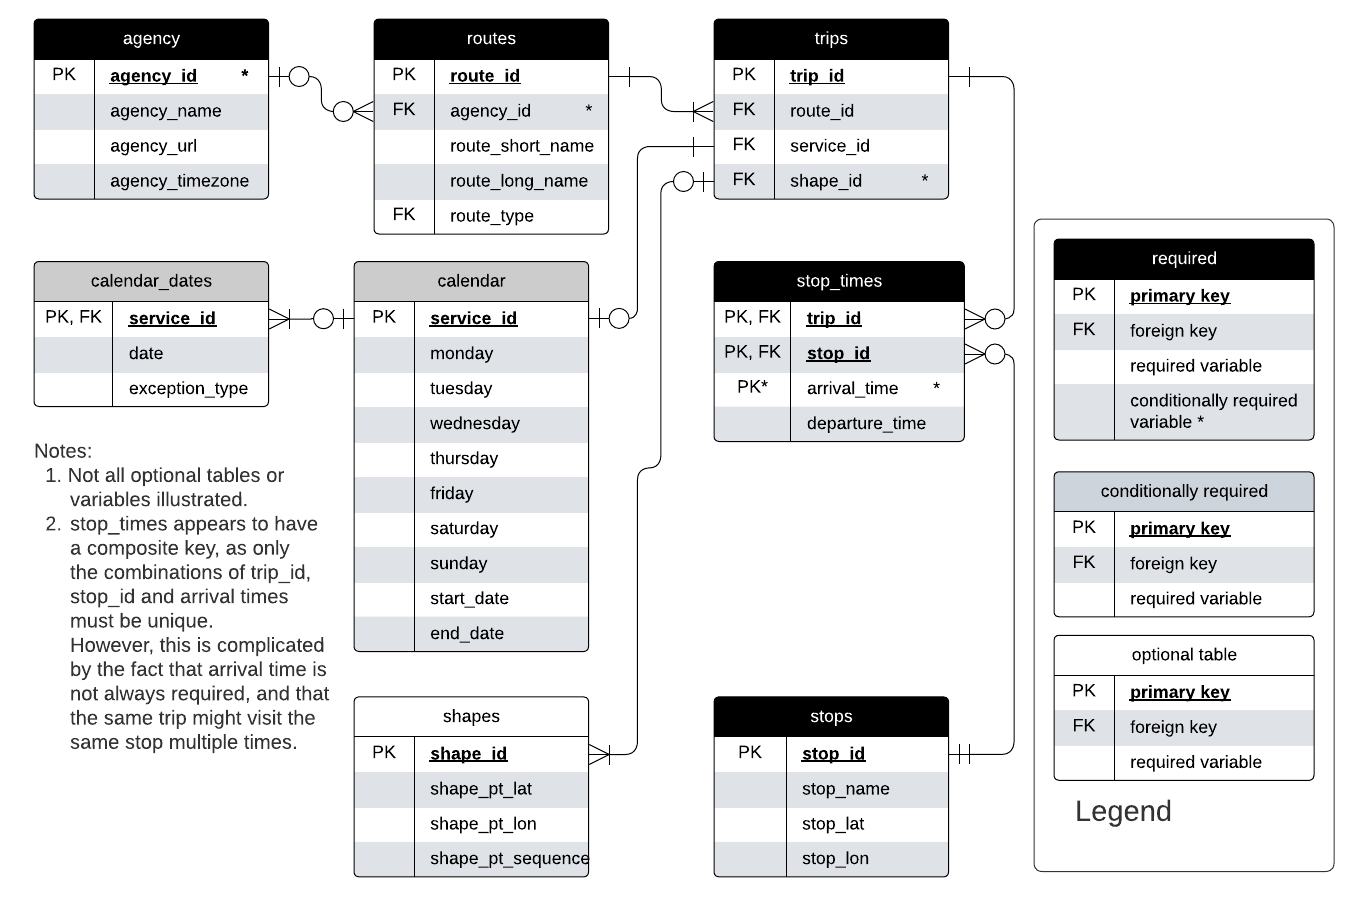
\includegraphics[width=1\linewidth]{graphics/GTFS} \caption{GTFS entity relationship diagram. Source: adapted by author from Alamri et al (2023) and the GTFS Schedule Reference (16/11/2023 revision).}\label{fig:GTFS_ERD}
\end{figure}

Figure @ref(fig:GTFS\_ERD) shows an Entity Relationship Diargram (ERD)
of the GTFS data structure. Each box represents a database table in the
GTFS, with table rows indicating the variables (columns) included in
each\footnote{ For example, each record in the `stops' table includes a
  value for stop\_id, stop\_name, stop\_lat and stop\_lon.}.
Relationships between the tables are indicated by the connecting lines,
and Primary Key (PK) and Foreign Key (FK) designations\footnote{ For
  example, stop\_id appears in the `stops' and `stop\_times' tables as a
  Primary Key and Foreign Key.}. `Crow's feet' indicate the
relationships between each table\footnote{ See
  https://i.stack.imgur.com/fxaAq.png for guide to the symbols. But, for
  example, the stops table is required, with the stop\_id field
  providing a unique (primary) key for every stop. Within the
  stop\_times table (which is also required) the stop\_id field is a
  foreign key. Each unique stop\_id can appear many times in the
  stop\_times table, but can appear only once in the stops table. In the
  stop\_times table each combination of trip\_id, stop\_id and arrival
  time must be unique (although see note 2!) meaning that these fields
  together represent a composite key.}.

GTFS now provides a mechanism for including individual transit systems
in many online products and analysis, including the Transit Score metric
itself. \citet{Wong:2013aa} provides another example of what can be done
with GTFS data, having developed code to calculate of some of the TCQSM
metrics\footnote{ Daily average headways, route length and stop numbers.}
for 50 transit operators. While the \citet{Wong:2013aa} open-source code
is readily available\footnote{
  https://github.com/jcwong86/GTFS\_Explore\_Tool} this is now 11 years
old and does not appear to be currently maintained. Future research may
involve reviewing this code and using it to analyse modern GTFS feeds.
However, in this paper the aim is more modest, being to use GTFS data to
calculate Currie and Senbergs' (2007) SI.

\hypertarget{the-transit-suppy-index}{%
\subsection{The Transit Suppy Index}\label{the-transit-suppy-index}}

A generalized form of the Transit Supply Index (SI) is shown in Equation
1\footnote{ Currie and Senbergs' (2007) focus was the context of
  Melbourne's Census Collection Districts (CCD) and calculations based
  on a week of transit service. CCDs predate the introduction of
  Statistical Areas 1, 2, 3, and 4 (SA1, SA2, SA3, SA4), and other
  geographical divisions currently used by the Australian Bureau of
  Statistics (ABS), which may be more familiar to readers from down
  under.}.

\[SI_{area, time} = \sum{\frac{Area_{Bn}}{Area_{area}}*SL_{n, time}}\]
In Equation 1:

\begin{enumerate}
\def\labelenumi{(\arabic{enumi})}
\tightlist
\item
  \(SI_{area, time}\) is the Supply Index for the area of interest and a
  given period of time;
\item
  \(Area_{Bn}\) is the buffer area for each stop (n) within the area of
  interest. In Currie and Senbergs (2007) this was based on a radius of
  400 metres for bus and tram stops, and 800 metres for railway
  stations;
\item
  \(Area_{area}\) is the area of the area of interest; and
\item
  \(SL_{n,time}\) is the number of transit arrivals for each stop for a
  given time period.
\end{enumerate}

An advantage of the SI is that it is a relatively simple number to
calculate, understand and explain. It describes the number of transit
arrivals at stops within an area of interest and time frame, multiplied
by a factor accounting for the proportion of the area of interest within
typical walking distances of each stop. Hence, more services, more stops
and higher frequencies increase the score. However, the SI does not
incorporate service span, speed or other elements of a transit service.
While these may be important to passenger experience, they might add
considerable complexity.

Simplicity is also helped by the way that the SI is additive, in that
\(SI_{area, time}\) scores can be aggregated to calculate an overall
score across multiple time periods or for a region encompassing multiple
areas of interest.

\hypertarget{methodology}{%
\section{Methodology}\label{methodology}}

This study developed a package with tools for calculating the SI from
GTFS data. R \citep{R-base}, a widely used and readily available
statistical programming language, was adopted for code development. The
package development setup and workflow described by \citet{wickham2023r}
was adopted in this study. Various existing packages were relied upon
including: the sf package \citep{R-sf} for geospatial analysis; the
tidyverse \citep{tidyverse2019}; gtfstools \citep{R-gtfstools}; and
tidytransit \citep{R-tidytransit}. Some code was adapted from examples,
vignettes and other documentation in the tidytransit, gtfstools and
other packages.

Two cases where used during the code development and testing such that
results might be generated for real GTFS data.\\
These cases were the Mornington Peninsula Tourist Railway GTFS feed and
the Public Transport Victoria (PTV) GTFS feed, both in Victoria,
Australia. Both were selected primarily for convenience, given that the
authors are familiar with the typical service patterns and geography.
Further cases were selected as leading, representative and contrasting
examples for the results reported here.

\hypertarget{mornington-penninsula-tourist-railway}{%
\subsection{Mornington Penninsula Tourist
Railway}\label{mornington-penninsula-tourist-railway}}

The Morning Peninsula Tourist Railway is located in the outer
south-eastern suburbs of Greater Melbourne. It runs on Sundays and
Wednesdays between Mornington (southwestern-most station) and Moorooduc,
with an intermediate stop at Tanti Park\footnote{https://transitfeeds.com/p/mornington-railway/806/latest/stops}.
A GTFS feed from 2018 was selected for the purposes of tests and
demonstrating the code and output. Australian Bureau of Statistics (ABS)
data was also used, primarily through the strayr and absmapsdata
packages \citep{r-strayr}. The Mornington Peninsular Statistical Area 3
(SA3) zone and the Statistical Area 1 (SA1) zones contained within it
were adopted as the areas of interest. These are shown in Figure
@ref(fig:mornington\_map\_ABS), together with the locations of the three
railway stations.

\begin{figure}
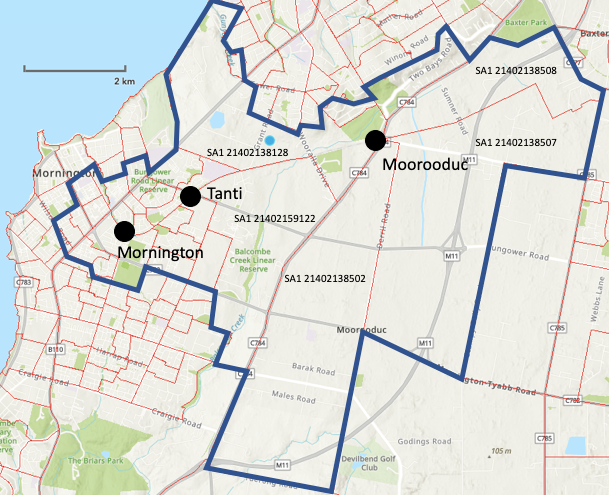
\includegraphics[width=1\linewidth]{graphics/mornington} \caption{SA1 zones and location of Mornington Tourist Railway Stations.}\label{fig:mornington_map_ABS}
\end{figure}

\hypertarget{public-transport-victoria-ptv}{%
\subsection{Public Transport Victoria
(PTV)}\label{public-transport-victoria-ptv}}

Larger scale testing was performed using the Victorian GTFS feed,
published by Public Transport Victoria (PTV), sourced via
\citet{transitfeeds_victoria:2023aa} for historical feeds. Again, ABS
data was used for the areas of interest.

\hypertarget{extensions}{%
\subsection{Extensions??}\label{extensions}}

Hourly ``Manhattan- and London-ised Indexes''

Tidytransit includes a sample GTFS feed from New York's MTA (including
the subway!), and so this was used for code tests were appropriate.

\hypertarget{results}{%
\section{Results}\label{results}}

\hypertarget{code-structure-and-output}{%
\subsection{Code structure and output}\label{code-structure-and-output}}

Developed code is available and documented on github
\citep{gtfssupplyindex_github}. The structure of the package and the
functions developed to generate each table are shown in Figure
@ref(fig:SI\_ERD). This indicates how the package takes input from three
files: a gtfs feed (gtfs.zip); a sf object describing the geometry of
the areas for which the SI is to be calculated; and a csv file defining
the buffer zone distances (in metres) for each route type\footnote{This
  file is included in the package.}.

\begin{figure}
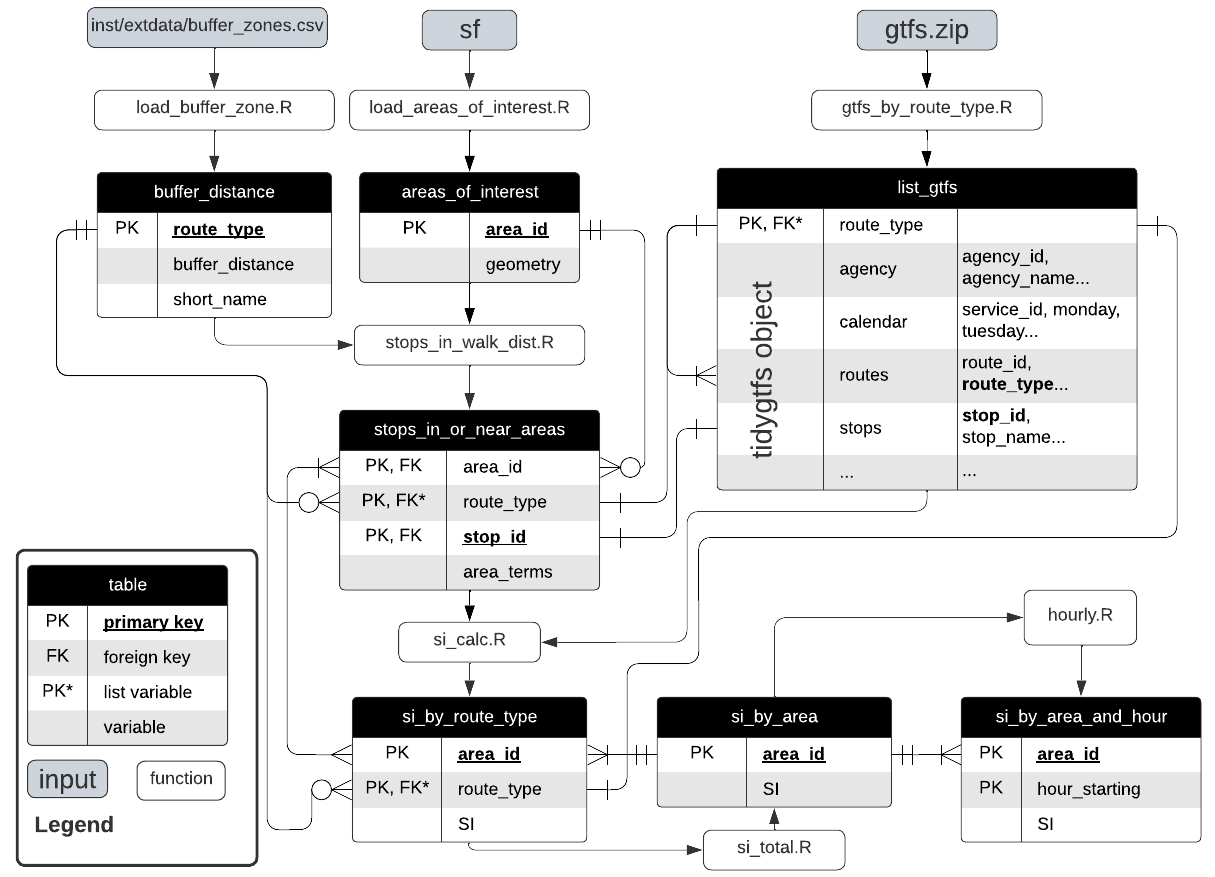
\includegraphics[width=1\linewidth]{graphics/SI_data_structure} \caption{Entity Relationship Diagram (ERD) showing the data structure and functions related to the gtfssupplyindex package}\label{fig:SI_ERD}
\end{figure}

The ultimate output is a si\_by\_area\_and\_hour table (Figure
@ref(fig:SI\_ERD), bottom right), which reports the SI score for each
hour of the day across dates specified by the user. The various
functions and their output and explained in the following, using the
Mornington Peninsula GTFS as an example.

\hypertarget{step-by-step-mornington-peninsula}{%
\subsection{Step-by-step: Mornington
Peninsula}\label{step-by-step-mornington-peninsula}}

This section presents outputs of the various functions for December
30th, 2018, using the Mornington Penninsula Tourist Railway GTFS feed
and SA1 zone boundaries. The individual steps involved in using the
gtfssupplyindex package are:

\begin{enumerate}
\def\labelenumi{(\arabic{enumi})}
\item
  loading the gtfs.zip file - the gtfs\_by\_route\_type function loads
  the gtfs data and splits it into a list (by route\_type) of tidygtfs
  objects, using the filter\_by\_route\_type function from the gtfstools
  package \citep{filter_GTFS_by_mode}.
\item
  loading geometry information about the areas of interest -
  geographical data about the areas of interest are loaded by the
  load\_areas\_of\_interest.R function into an sf object, using the sf
  package \citep{R-sf} . The resultant areas\_of\_interest table
  contains each area\_id and its associated geometry. Data about buffer
  zones, specifically the walking distance threshold assigned to each
  route\_type (mode) is then loaded, again through a function
  (load\_buffer\_zone.R). The package includes this information in a csv
  file, in which the buffer zone is defined in metres.
\item
  calculating which stops are within the catchment walking distance of
  which areas, which is achieved using the stops\_in\_walk\_dist
  function. However, this is complicated by the need to have different
  buffer distances for each route\_type, and to only include those parts
  of the walking catchment that are within each area of interest. The
  calculation involves: (1) looking up the buffer\_distance\_length
  specific to each route\_type; (2) transforming from latitude and
  longitude into metres and determining the area; (3) drawing circles
  around each stop, with the radius equal to the buffer distance, and
  intersecting these with the areas\_of\_interest (see Figure
  @ref(fig:calculate\_stop\_in\_or\_near\_areas\_verbose)); (4)
  calculating the \(area_{Bn}\) terms are for each combination of
  stop\_id and area\_id; and then reporting the overall area terms for
  each area\_of\_interest (\(Area_{Bn} / Area_{Area}\)), as shown in
  Table \ref@(tab:calculate\_stop\_in\_or\_near\_areas).
\end{enumerate}

\begin{Shaded}
\begin{Highlighting}[]
\NormalTok{stops\_in\_or\_near\_areas }\OtherTok{\textless{}{-}}\NormalTok{ gtfssupplyindex}\SpecialCharTok{:::}\FunctionTok{stops\_in\_walk\_dist}\NormalTok{(}
  \AttributeTok{list\_gtfs =}\NormalTok{ list\_gtfs, }
  \AttributeTok{areas\_of\_interest =}\NormalTok{ areas\_of\_interest,}
  \AttributeTok{EPSG\_for\_transform =} \DecValTok{28355}\NormalTok{, }
  \AttributeTok{verbose =} \ConstantTok{TRUE}
\NormalTok{)}
\end{Highlighting}
\end{Shaded}

\begin{figure}
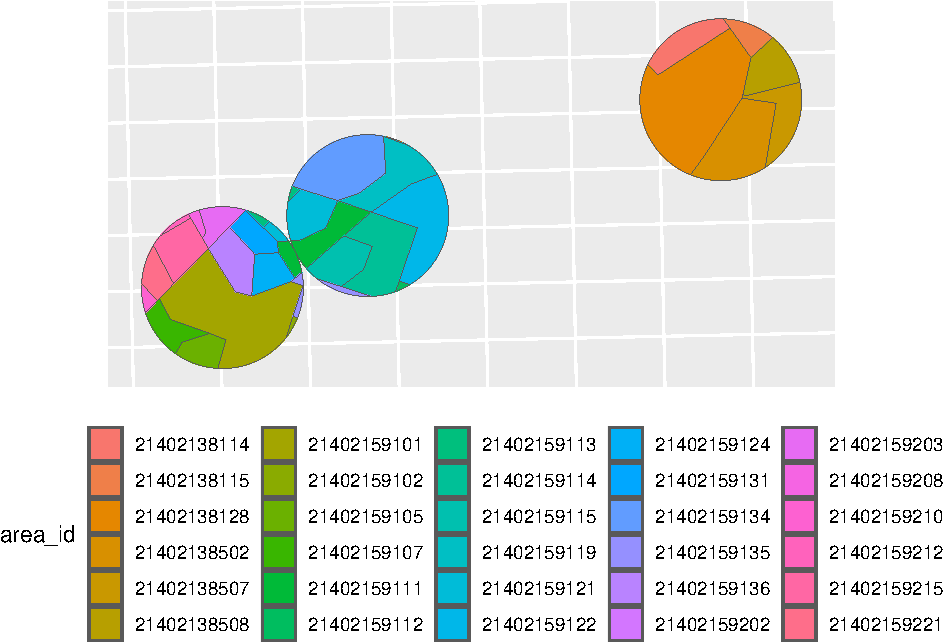
\includegraphics[width=1\linewidth]{Leveraging_GTFS_to_assess_transit_supply_Transport_Geography_files/figure-latex/calculate_stop_in_or_near_areas_verbose-1} \caption{Step 3, part 4, stop catchments for the Mornington Penninsula Tourist Railway, showing intersections with SA1 zones}\label{fig:calculate_stop_in_or_near_areas_verbose}
\end{figure}

\begin{table}

\caption{\label{tab:calculate_stop_in_or_near_areas}'Rail' element of the stops in or near areas list for the Mornington Pennisula datasets, first six entries}
\centering
\begin{tabular}[t]{l|l|r}
\hline
stop\_id & area\_id & area\_terms\\
\hline
1388695887 & 21402159101 & 0.7999912\\
\hline
1388695887 & 21402159102 & 0.0168220\\
\hline
1388695887 & 21402159105 & 0.6779951\\
\hline
1388695887 & 21402159107 & 0.6453927\\
\hline
1388695887 & 21402159111 & 0.2011127\\
\hline
1388695887 & 21402159113 & 0.1081424\\
\hline
\end{tabular}
\end{table}

\begin{enumerate}
\def\labelenumi{(\arabic{enumi})}
\setcounter{enumi}{3}
\tightlist
\item
  Calculating SI scores for a given time period, using the si\_calc.R
  function. This adapts code from an article included in the tidytransit
  package \citep{tidytransit_departure_timetable} to calculate the
  number of arrivals in a given time period, and then combines this with
  the area terms to calculate the SI score. The si\_total.R function
  aggregates the SI scores across all modes, although the Mornington
  Penninsula example presented here only includes rail services. Hourly
  values can likewise be generated using the hourly.R function which
  runs , giving the results shown in Table
  @ref(tab:SI\_mornington\_20181230\_output)and mapped in Figure
  @ref(fig:SI\_mornington\_20181230\_output).
\end{enumerate}

The ultimate output, showing the SI scores for each hour, isshown in
Table @ref(tab:SI\_mornington\_20181230\_output) and mapped in Figure
@ref(fig:SI\_mornington\_20181230\_output).

\begin{table}

\caption{\label{tab:SI_mornington_20181230_output}Mornington Penninsula Tourist Railway hourly SI values for December 30, 2018, for first 6 SA1 zones}
\centering
\begin{tabular}[t]{l|r|r|r|r|r|r}
\hline
area\_id & 10:00 & 11:00 & 12:00 & 13:00 & 14:00 & 15:00\\
\hline
21402138114 & 0 & 0.5 & 0.5 & 0 & 0.5 & 0.5\\
\hline
21402138115 & 0 & 0.1 & 0.1 & 0 & 0.1 & 0.1\\
\hline
21402138128 & 0 & 0.2 & 0.2 & 0 & 0.2 & 0.2\\
\hline
21402138502 & 0 & 0.0 & 0.0 & 0 & 0.0 & 0.0\\
\hline
21402138507 & 0 & 0.0 & 0.0 & 0 & 0.0 & 0.0\\
\hline
21402138508 & 0 & 0.0 & 0.0 & 0 & 0.0 & 0.0\\
\hline
\end{tabular}
\end{table}

\begin{figure}
\centering
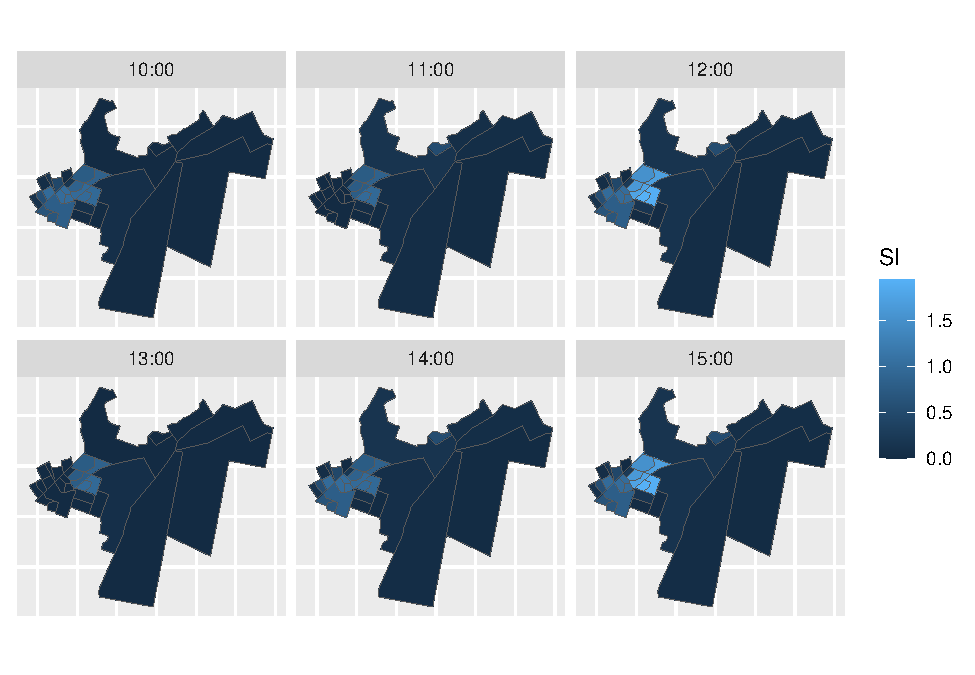
\includegraphics{Leveraging_GTFS_to_assess_transit_supply_Transport_Geography_files/figure-latex/SI_mornington_20181230_output-1.pdf}
\caption{Mornington Penninsula Tourist Railway hourly SI values for
December 30, 2018}
\end{figure}

The results meet expectations, with higher scores for SA1 zones closer
to the three stations. Hand calculation for SA1 21402159136, which is
close to the Mornington Station, to confirm the results is relatively
trivial. By inspection, all of SA1 21402159136 (shown in purple in
Figure @ref(fig:calculate\_stop\_in\_or\_near\_areas\_verbose) is within
an 800 metre walking distance of Mornington Station, meaning that
\(Area_{Bn} / Area_{area} = 1\). The SI scores for each hour are
therefore equal to the number of arrivals in each hour. Table
@ref(tab:mornington\_hand\_check) shows the scores calculated by the
function, which matches the pattern of arrivals at 10:47am, 12:12pm,
2:02pm and 3:27pm\footnote{See
  https://transitfeeds.com/p/mornington-railway/806/latest/stops}.

\begin{table}

\caption{\label{tab:mornington_hand_check}Mornington Penninsula Tourist Railway hourly SI values for December 30, 2018, for SA1 zone 21402159136}
\centering
\begin{tabular}[t]{l|r|r|r|r|r|r}
\hline
area\_id & 10:00 & 11:00 & 12:00 & 13:00 & 14:00 & 15:00\\
\hline
21402159136 & 1 & 0 & 1 & 0 & 1 & 1\\
\hline
\end{tabular}
\end{table}

\hypertarget{greater-melbourne---october-2023}{%
\subsection{Greater Melbourne - October
2023}\label{greater-melbourne---october-2023}}

As a further example, hourly SI scores were calculated for all SA1 2021
zones within Greater Melbourne on Tuesday 10th, Saturday 14th and Sunday
15th October, 2023. These dates were selected so as to match the typical
census timing of a Tuesday early in October, although 2023 is not
actually a census year. GTFS data was obtained from
\citet{transitfeeds_victoria:2023aa}, with the October 6, 2023 dataset
selected\footnote{Minor adjustments were made to this dataset to remove
  duplicate stop\_ids from the stops.txt file}. SI scores by hour for
SA1 zones in the centre of Melbourne (shown in Figure @ref(CBD\_map)) on
Tuesday 10th October are shown in Figure
@ref(Melbourne\_CBD\_map\_231010),

\begin{figure}
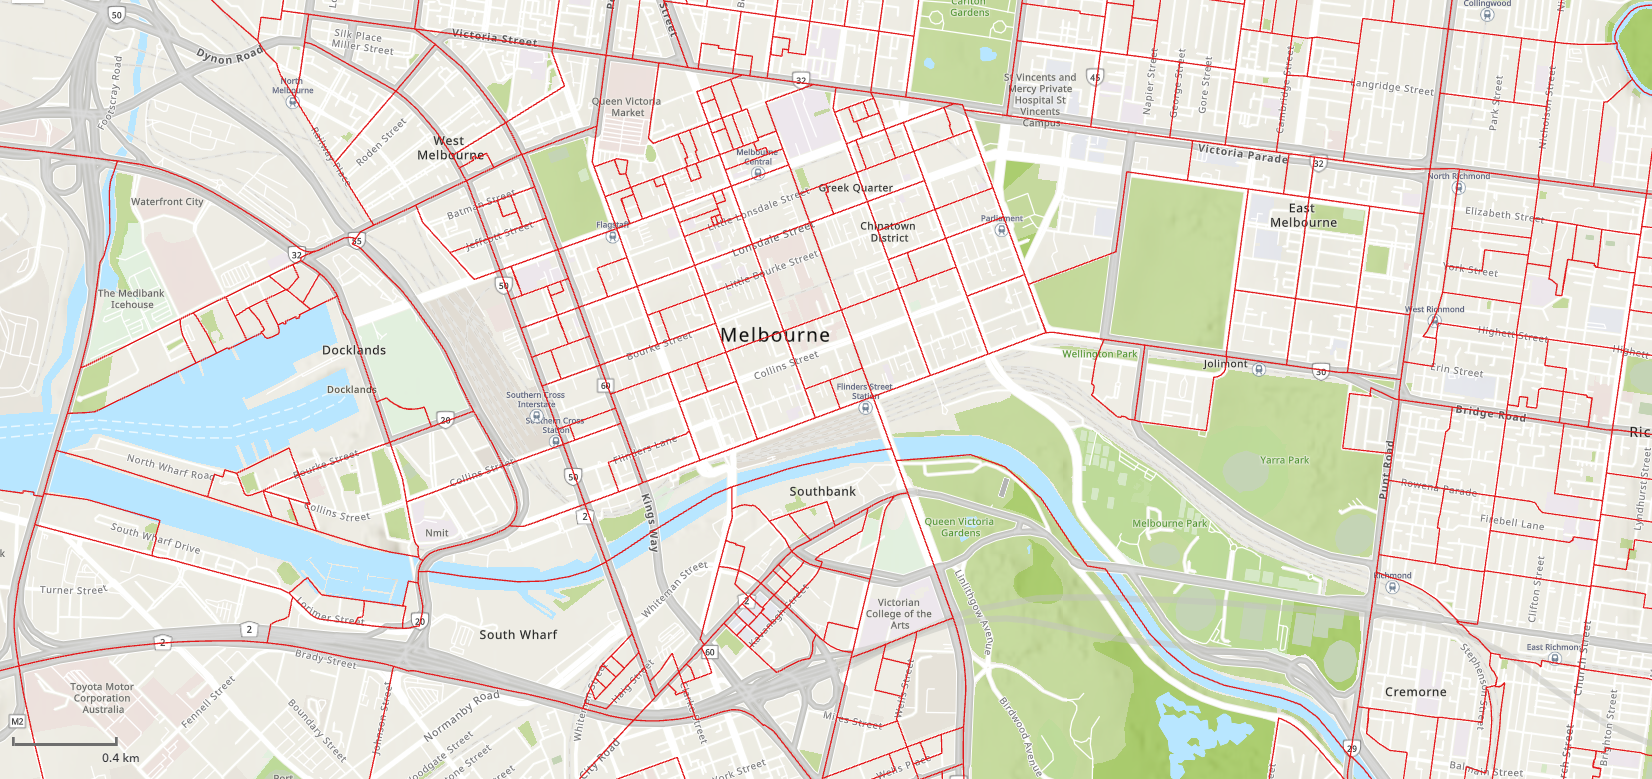
\includegraphics[width=1\linewidth]{graphics/Melbourne_cbd} \caption{SA1 zones and location of Mornington Tourist Railway Stations.}\label{fig:CBD_map}
\end{figure}

\begin{figure}
\centering
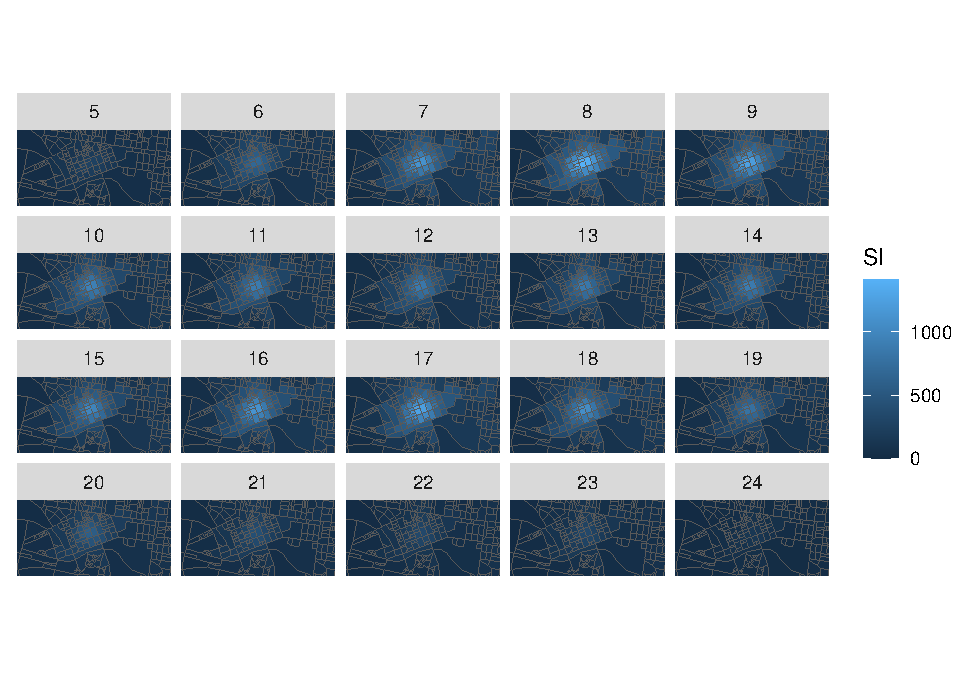
\includegraphics{Leveraging_GTFS_to_assess_transit_supply_Transport_Geography_files/figure-latex/Melbourne_CBD_map_231010-1.pdf}
\caption{Victorian GTFS and SA1 zones near the Melbourne CBD, SI values
for October 10, 2023, by hour between 5am and 1am}
\end{figure}

The results shown in Figure @ref(Melbourne\_CBD\_map\_231010) meet
expectations, with higher SI scores shown in the Central Business
District (CBD), where there are the five stations that make up the City
Loop\footnote{Flinders Street Station, Southern Cross Station, Flagstaff
  Station, Melbourne Central Station and Parliament Station.}, and where
many tram and bus routes converge. The SI scores are highest during the
day, especially in the morning and afternoon peak periods around 7-9am
and 4-7pm, reflecting the typical service peaks.

\hypertarget{by-mode}{%
\subsubsection{By mode}\label{by-mode}}

SI scores were also obtained for each mode separately. Scores for the
whole day on Tuesday October 10th, 2023 are shown in Figure
@ref(Melbourne\_231010\_by\_mode).

Figure @ref(Melbourne\_231010\_by\_mode) indicates how the central city
is serviced by: - buses that mostly travel along the Latrobe and Queen
Street corridors, many of which travel east-west along Victoria Street
to/from the north-east; - rail services stopping at City Loop stations;
and - tram services, most of which running north-south along the
Swanston Street corridor.

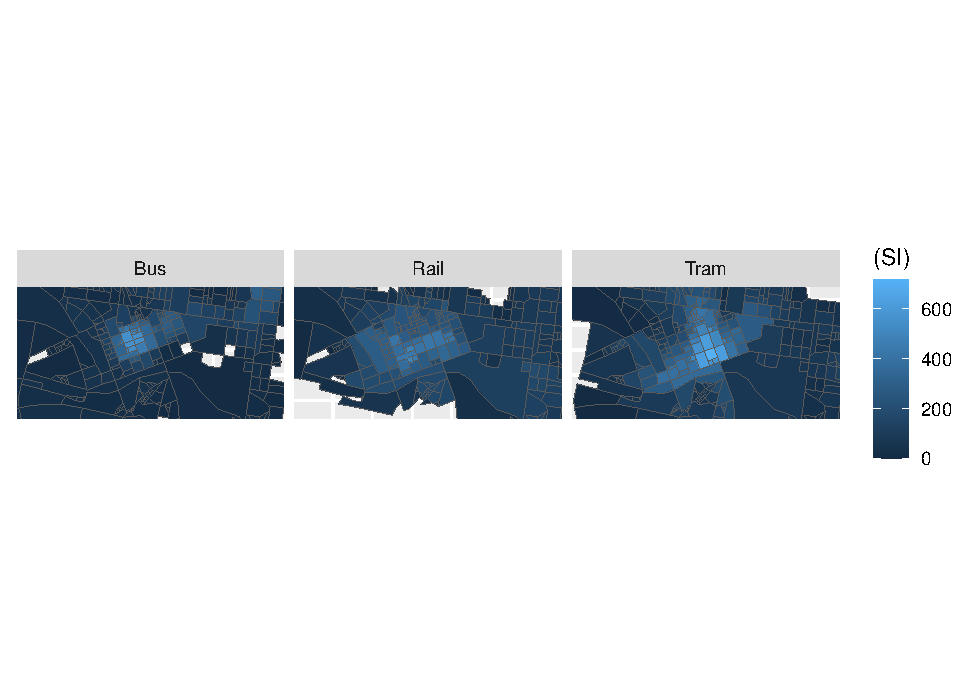
\includegraphics{Leveraging_GTFS_to_assess_transit_supply_Transport_Geography_files/figure-latex/Melbourne_231015_by_mode-1.pdf}
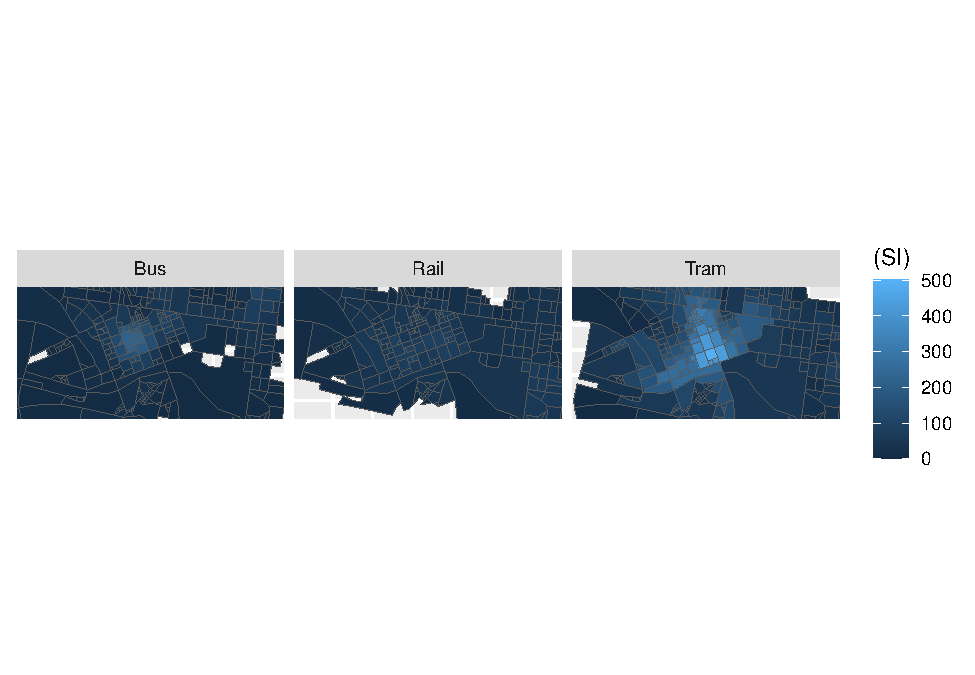
\includegraphics{Leveraging_GTFS_to_assess_transit_supply_Transport_Geography_files/figure-latex/Melbourne_231015_by_mode-2.pdf}
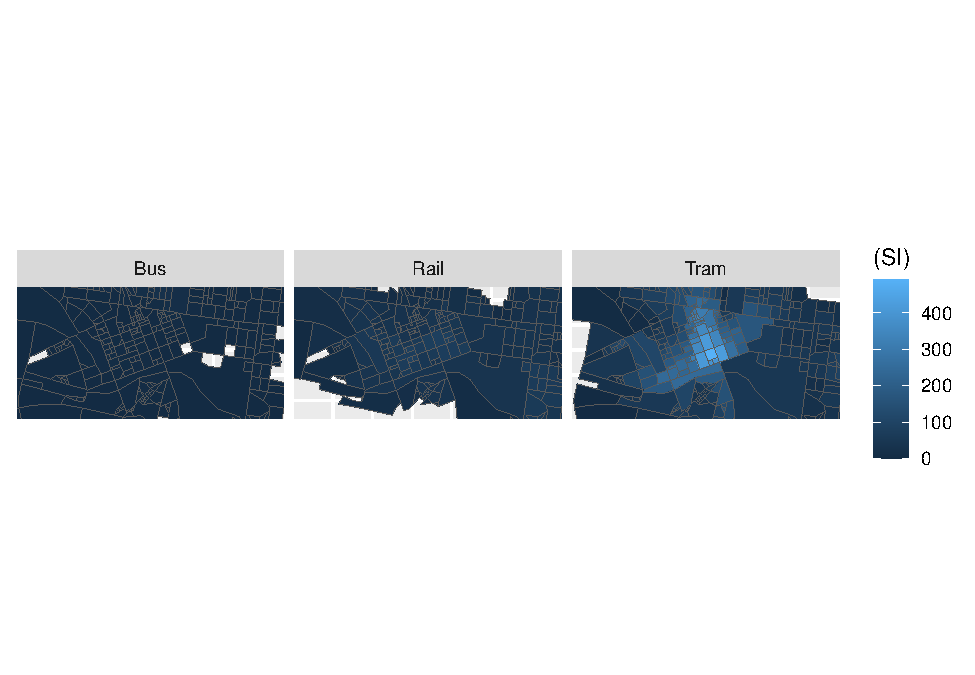
\includegraphics{Leveraging_GTFS_to_assess_transit_supply_Transport_Geography_files/figure-latex/Melbourne_231015_by_mode-3.pdf}

Figure @ref(Melbourne\_231015\_by\_mode) shows a similar plot, but for
Sunday October 15th, 2023. However, in this case the bus scores appear
very low. While Sunday bus services in the CBD are generally much less
frequent on Sundays than on other days, further investigation suggests
that strike action had been planned around that time by transit
workers\citep{Hannaford_2023}. While it is unclear what normal services
had been officially cancelled around that time, it appears likely that
Sunday bus services may have been cut so as to have some replacement bus
capacity available on other days. Regardless, this suggests that the
October 2023 services reported above may not actually be representative
of typical conditions in Melbourne. Hence, in the following section a
similar analysis is shown for July 2023 instead.

\hypertarget{greater-melbourne---july-2023}{%
\subsection{Greater Melbourne - July
2023}\label{greater-melbourne---july-2023}}

\hypertarget{central-business-district-cbd}{%
\subsubsection{Central Business District
(CBD)}\label{central-business-district-cbd}}

\hypertarget{clayton}{%
\subsubsection{Clayton}\label{clayton}}

\hypertarget{local-government-areas}{%
\subsubsection{Local Government Areas}\label{local-government-areas}}

\hypertarget{patterns}{%
\subsubsection{Patterns}\label{patterns}}

\hypertarget{trends}{%
\subsubsection{Trends}\label{trends}}

\hypertarget{extensions-1}{%
\section{Extensions}\label{extensions-1}}

\hypertarget{melbourne-cbd-index}{%
\subsection{Melbourne CBD Index}\label{melbourne-cbd-index}}

\hypertarget{new-york-index}{%
\subsection{New York Index}\label{new-york-index}}

\hypertarget{london-index}{%
\subsection{London Index}\label{london-index}}

\hypertarget{discussion-and-conclusions}{%
\section{Discussion and conclusions}\label{discussion-and-conclusions}}

\renewcommand\refname{References}
\bibliography{References.bib, packages.bib}


\end{document}
